\documentclass[11pt]{article}
\usepackage{my_syllabus}


 \author{Joshua Bowles}
\title{Possible Research Topics\\
\small Eng 2020 Spring 2010}
\date{\today}

\begin{document}
\maketitle

%\includegraphics[width=1in]{madscientistmuppet}\includegraphics[width=2in]{UVU_Horizontal_Mark_1-color}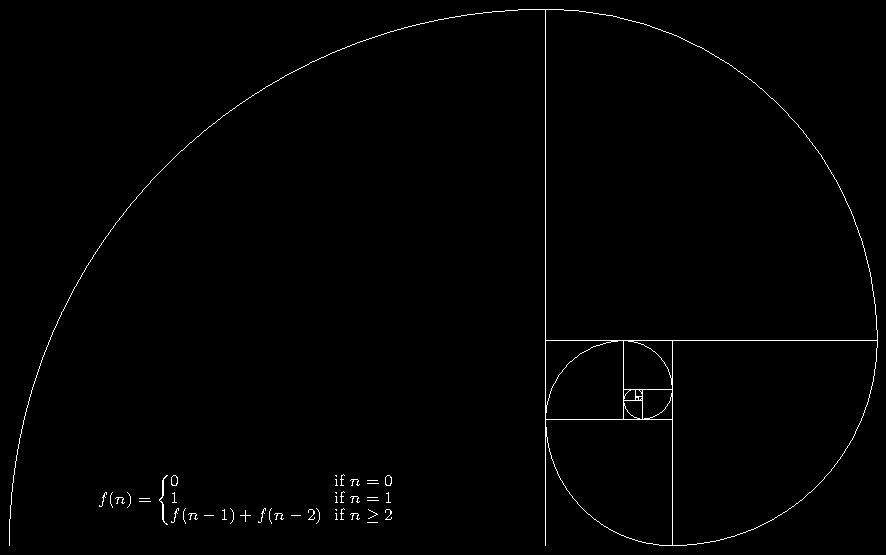
\includegraphics[width=2in]{fibonacci-spiral}\includegraphics[width=1in]{Rplot001}

\section{Possible Research Topics}
\begin{enumerate}
\item Mathematics of symmetry and Fibonacci patterns in nature
\item Mathematics of probability
\item Mathematics of encryption and security
\item Economics of personal and corporate debt
\item Biology of stem cells, e.g., differentiation and reverse engineering\footnote{\emph{Many people} write papers on this topic.}
\item Quantum computers, quantum computation, and the theory of quantum consciousness
\item Science of alternative energy\footnote{Again, many people write on this subject.}
\item Biographical life of a scientist---Newton, Einstein, Galileo, Galois, Abels, Cantor, Turing, Boole, Godel\ldots{}
\item Symmetry and Fibonacci patterns art: real science or wishful perception?
\item Statistics and Probability in medicine, insurance, game shows, gambling, physics, marketing
\item Encryption and security
\item Philosophy of science; science-religion connections/divides, etc.\ldots
\item Literature and consciousness
\item Artificial Intelligence and Gaming
\item Gaming and Social Networks
\item Social Networking and `Hooking up'
\item Do animals have anything like human language? (other mammals? primates? bees?)
\item Homosexuality: nature or nurture?
\item Is racism a behavior that used to be an evolutionary advantage?
\item {\bf the list goes on\ldots}
\end{enumerate}

\subsection{Comment}  
You should find something that engages you, or something that you think is crazy and would never be allowed to write about for a college. The point of attending a University\footnote{Besides the obvious and beaurocratic goal of \emph{making more money.}} is to get the chance to have a \emph{transformative experience}. You can have a good experience in this class, and do interesting research, if you pick topics that are really cool.

\section{Research}
\subsection{Databases}\begin{itemize}  
\item Research tools accessible at the \href{http://www.uvu.edu/library/researchtools/index.html}{UVU-Library}
\item \href{http://www.uvu.edu/library/guides/index.html}{Research guides} by topic at UVU library
\item \href{http://www.uvu.edu/library/researchtools/electronic_encyclopedias.html}{Electronic Encyclopedias and Dictionaries}
\item JSTOR 
\item ScienceDirect 
\item ERIC 
\item Academic Search Premier 
\item Project Muse
\end{itemize}

\subsection{Other Places}
\begin{itemize}
\item \href{http://mitpress.mit.edu}{MIT Press} 
\item \href{http://arxiv.org}{Cornell ArXiv} 
\item \href{http://plato.stanford.edu/}{Stanford Encyclopedia of Philosophy} 
\item Academic web pages of \href{http://www.uvu.edu/profpages/profiles/show/user_id/530}{professors} for downloadable papers\footnote{Make sure these sites are connected to a University or College---as the example here shows, if you are on-line!}
\end{itemize}

\subsection{Organizations and Websites}
\begin{itemize}
\item\href{http://www.amwa.org/}{American Medical Writers Association}
\item\href{http://www.attw.org/}{Association of Teachers of Technical Writing}
\item\href{http://www.ieeepcs.org/}{IEEE Professional Communication Society}
\item\href{http://nasw.org/}{National Association of Science Writers}
\item\href{http://www.stc.org/}{Society for Technical Communication}
\end{itemize}

\end{document}  
